\begin{topic}{separable-state}{separable state}
    Let $\mathcal{H}_1, \ldots, \mathcal{H}_n$ be the Hilbert spaces of $n$ quantum systems. A state $\ket{\psi} \in \mathcal{H}_1 \otimes \cdots \otimes \mathcal{H}_n$ is \emph{separable} if it can be written as $\ket{\psi} = \ket{\psi_1} \otimes \cdots \otimes \ket{\psi_n}$ for some $\ket{\psi}_i \in \mathcal{H}_i$.
\end{topic}

\begin{topic}{entangled-state}{entangled state}
    Let $\mathcal{H}_1, \ldots, \mathcal{H}_n$ be the Hilbert spaces of $n$ quantum systems. A state $\ket{\psi} \in \mathcal{H}_1 \otimes \cdots \otimes \mathcal{H}_n$ is \emph{entangled} if it is not \tref{separable-state}{separable}, that is, if it cannot be written as $\ket{\psi} = \ket{\psi_1} \otimes \cdots \otimes \ket{\psi_n}$ for some $\ket{\psi}_i \in \mathcal{H}_i$.
\end{topic}

\begin{topic}{density-matrix}{density matrix}
    Let $\mathcal{H}$ be the Hilbert space of a quantum system. A \emph{density matrix}, also known as \emph{density operator}, on $\mathcal{H}$ is a bounded operator $\rho \colon \mathcal{H} \to \mathcal{H}$ which is positive-definite and has trace $\tr(\rho) = 1$.
\end{topic}

\begin{example}{density-matrix}
    In general, any density matrix $\rho$ can be written as
    \[ \rho = \sum_{i = 1}^{m} p_i \ket{\psi_i} \bra{\psi_i} \]
    for some $\ket{\psi_i} \in \mathcal{H}$ and $0 \le p_i \le 1$ with $\sum_{i = 1}^{m} p_i = 1$. If $p_i = 1$ for some $i$, then $\rho$ is called \tref{pure-state}{pure}. Otherwise, $\rho$ is called \tref{mixed-state}{mixed}.
\end{example}

\begin{topic}{pure-state}{pure state}
    Let $\mathcal{H}$ be the Hilbert space of a quantum system. A \emph{pure state} is a \tref{density-matrix}{density matrix} of the form $\rho = \ket{\psi} \bra{\psi}$ for some $\ket{\psi} \in \mathcal{H}$.
\end{topic}

\begin{topic}{mixed-state}{mixed state}
    Let $\mathcal{H}$ be the Hilbert space of a quantum system. A \emph{mixed state} is a \tref{density-matrix}{density matrix} which is not a \tref{pure-state}{pure state}.
\end{topic}

\begin{topic}{purity}{purity}
    The \emph{purity} of a \tref{density-matrix}{density matrix} $\rho$ is the trace of its square, that is, $\tr(\rho^2)$.
\end{topic}

\begin{example}{purity}
    When $\rho = \ket{\psi} \bra{\psi}$ is \tref{pure-state}{pure}, the purity of $\rho$ is $\tr(\rho^2) = \braket{\psi}{\psi}^2 = 1$. In general, the purity satisfies $(\dim \mathcal{H})^{-1} \le \tr(\rho^2) \le 1$.
\end{example}

\begin{example}{purity}
    The purity of a density matrix $\rho$ is conserved under unitary transformations. That is, for any unitary transformation $U$,
    \[ \tr((U \rho U^\dag)^2) = \tr(\rho^2) \]
    using that $UU^\dag = U^\dag U = 1$ and the cyclic property of the trace.
\end{example}

\begin{topic}{reduced-density-matrix}{reduced density matrix}
    Let $\mathcal{H}_1$ and $\mathcal{H}_2$ be the Hilbert spaces of two quantum systems. Given a \tref{density-matrix}{density matrix} $\rho$ on $\mathcal{H}_1 \otimes \mathcal{H}_2$, the \emph{reduced density matrix} of $\rho$ on $\mathcal{H}_1$ is the density matrix
    \[ \rho_1 = \tr_2(\rho) \]
    given by the partial trace over $\mathcal{H}_2$. Explicitly, the partial trace $\tr_2$ is given by
    \[ \tr_2 \left( \ket{\psi} \bra{\psi'} \otimes \ket{\varphi} \bra{\varphi'} \right) = \braket{\varphi'}{\varphi} \cdot \ket{\psi} \bra{\psi'} \]
    for all $\ket{\psi}, \ket{\psi'} \in \mathcal{H}_1$ and $\ket{\varphi}, \ket{\varphi'} \in \mathcal{H}_2$ and extended linearly.
\end{topic}

\begin{topic}{no-cloning-theorem}{no-cloning theorem}
    Consider two quantum systems, $A$ and $B$, with a common Hilbert space $\mathcal{H}_A = \mathcal{H}_B = \mathcal{H}$. The \emph{no-cloning theorem} states that there exists no unitary operation $U$ on $\mathcal{H}_A \otimes \mathcal{H}_B$ such that
    \[ U (\ket{\psi} \otimes \ket{\phi}) = \ket{\psi} \otimes \ket{\psi} \]
    for all $\ket{\psi} \in \mathcal{H}$ and any $\ket{\phi} \in \mathcal{H}$.
\end{topic}

\begin{example}{no-cloning-theorem}
    \begin{proof}
        If such an operation $U$ would exist, it would not be linear in $\ket{\psi}$, and hence would not be unitary.
    \end{proof}
\end{example}

\begin{topic}{uncertainty-principle}{uncertainty principle}
    Let $A$ and $B$ be two \tref{observable}{observables} on a Hilbert space $\mathcal{H}$. For any state $\ket{\psi} \in \mathcal{H}$, write
    \[ \Delta A = A - \langle A \rangle \quad \textup{ where} \quad \langle A \rangle = \bra{\psi} A \ket{\psi} \]
    and denote by
    \[ \langle (\Delta A)^2 \rangle = \bra{\psi} (A - \bra{\psi} A \ket{\psi})^2 \ket{\psi} = \bra{\psi} A^2 \ket{\psi} - \bra{\psi} A \ket{\psi}^2 \]
    the \textit{variance} of $A$. The \emph{uncertainty principle} states that
    \[ \langle (\Delta A)^2 \rangle \langle (\Delta B)^2 \rangle \ge \left(\frac{1}{2 i} \langle [A, B] \rangle \right)^2 \]
    for all states $\ket{\psi} \in \mathcal{H}$, where $[A, B] = AB - BA$ denotes the commutator of $A$ of $B$.
\end{topic}

\begin{example}{uncertainty-principle}
    Let $A = x$ and $B = p = - i \hbar \tfrac{\partial}{\partial x}$ be the position and momentum operators of a particle. The uncertainty principle reduces to the \textit{Heisenberg uncertainty principle}
    \[ \sigma_x^2 \sigma_p^2 \ge \left(\frac{1}{2 i} \langle [x, p] \rangle \right)^2 = \frac{\hbar^2}{4} \]
    since $[x, p] = i \hbar$.
\end{example}

\begin{topic}{lenz-ising-model}{Lenz--Ising model}
    The \emph{Lenz--Ising model} is an \tref{COM:qubit}{$n$-qubit} quantum system with Hamiltonian
    \[ H = - \sum_{\substack{i, j = 1 \\ i \ne j}}^{n} J_{ij} \sigma_z^{(i)} \sigma_z^{(j)} - \mu \sum_{j = 1}^{n} h_j \sigma_z^{(j)} \]
    where
    \begin{itemize}
        \item $\sigma_z^{(i)}$ is $\left(\begin{smallmatrix} 1 & 0 \\ 0 & -1 \end{smallmatrix}\right)$ acting on the $i$-th qubit,
        \item $J_{ij}$ are the \textit{coupling strengths},
        \item $h_j$ are the \textit{external magnetic field strengths},
        \item $\mu$ is the \textit{magnetic moment}.
    \end{itemize}
\end{topic}

\begin{topic}{schrodinger-equation}{Schrödinger equation}
    The \emph{Schrödinger equation} describes the time-evolution of the state $\psi(t) \in \mathcal{H}$ of a quantum system with Hilbert space $\mathcal{H}$ and Hamiltonian $H$,
    \[ i \hbar \frac{d}{dt} \psi = H \psi . \]
\end{topic}

\begin{topic}{von-neumann-equation}{von Neumann equation}
    The \emph{von Neumann equation} describes the time-evolution of the \tref{mixed-state}{mixed state} $\rho(t)$ of a quantum system with Hilbert space $\mathcal{H}$ and Hamiltonian $H$,
    \[ i \hbar \frac{d}{dt} \rho = [H, \rho] . \]
\end{topic}

\begin{topic}{observable}{observable}
    An \emph{observable} is a self-adjoint operator on the Hilbert space $\mathcal{H}$ of a quantum system (corresponding to a physical quantity that can be measured).
\end{topic}

\begin{example}{observable}
    The Hamiltonian $H$ of a quantum system is an observable corresponding to the total energy of the system.
\end{example}

\begin{topic}{ehrenfest-theorem}{Ehrenfest's theorem}
    Consider a quantum system with Hamiltonian $H$ and let $A$ be some \tref{observable}{observable}. The \emph{(generalized) Ehrenfest's theorem} states that 
    % \[ \frac{d}{dt} \bra{\psi} A \ket{\psi} = \frac{1}{i \hbar} \bra{\psi} [A, H] \ket{\psi} + \bra{\psi} \frac{\partial A}{\partial t} \ket{\psi} . \]
    \[ \frac{d}{dt} \langle A \rangle = \frac{1}{i \hbar} \langle [A, H] \rangle + \left\langle \frac{\partial A}{\partial t} \right\rangle , \]
    where $\langle A \rangle$ denotes the expected value $\bra{\psi} A \ket{\psi}$ of $A$.
\end{topic}

\begin{example}{ehrenfest-theorem}
    Consider the quantum system consisting of a $1$-dimensional particle with mass $m$, with Hamiltonian
    \[ H = \frac{\hbar^2}{2 m} \frac{\partial^2}{\partial x^2} + V(x) . \]
    From Ehrenfest's theorem follows that
    \[ \frac{d}{dt} \langle x \rangle = \frac{1}{i \hbar} \langle [x, H] \rangle + \left\langle \frac{\partial x}{\partial t} \right\rangle = \left\langle - \frac{i \hbar}{m} \frac{\partial}{\partial x} \right\rangle = \frac{\langle p \rangle}{m} , \]
    where $p = -i \hbar \frac{\partial}{\partial x}$ is the momentum operator. Similarly, we have
    \[ \frac{d}{dt} \langle p \rangle = \frac{1}{i \hbar} \langle [p, H] \rangle + \left\langle \frac{\partial p}{\partial t} \right\rangle = \left\langle - \frac{\partial}{\partial x} V(x) \right\rangle . \]
    Combined, we find that
    \[ m \frac{d^2}{d t^2} \langle x \rangle = \left\langle - \frac{\partial}{\partial x} V(x) \right\rangle \]
    which corresponds to the classical equation of motion for the particle.
\end{example}

\begin{topic}{coherent-spin-state}{coherent spin state}
    Let a quantum system be given with angular momentum operators $S = (S_x, S_y, S_z)$, satisfying the usual cyclic commutation relations
    \[ [S_x, S_y] = i S_z, \quad [S_y, S_z] = i S_x, \quad [S_z, S_x] = i S_y . \]
    For any unit vector $v = (v_x, v_y, v_z) \in \RR^3$, a \emph{coherent spin state} of the system in the direction of $v$ is an eigenstate of the operator $v \cdot S = v_x S_x + v_y S_y + v_z S_z$.
\end{topic}

\begin{example}{coherent-spin-state}
    Consider a spin-$\tfrac{1}{2}$ system, that is, a two-dimensional quantum system $\mathcal{H}$ with operators
    \[ S_x = \begin{pmatrix} 0 & \tfrac{1}{2} \\ \tfrac{1}{2} & 0 \end{pmatrix}, \quad S_y = \begin{pmatrix} 0 & - \tfrac{i}{2} \\ \tfrac{i}{2} & 0 \end{pmatrix}, \quad S_z = \begin{pmatrix} \tfrac{1}{2} & 0 \\ 0 & - \tfrac{1}{2} \end{pmatrix} . \]
    The coherent spin states in the direction of $v = (0, 0, 1)$ are $\ket{\uparrow} = \left(\begin{smallmatrix} 1 \\ 0 \end{smallmatrix}\right)$ and $\ket{\downarrow} = \left(\begin{smallmatrix} 0 \\ 1 \end{smallmatrix}\right)$.

    Combining $n$ spin-$\tfrac{1}{2}$ systems, we obtain a spin-$\tfrac{n}{2}$ system $\mathcal{H}^{\otimes n}$, with operators
    \[ S_x = \sum_{i = 1}^{n} S_x^{(i)}, \quad S_y = \sum_{i = 1}^{n} S_y^{(i)}, \quad S_z = \sum_{i = 1}^{n} S_z^{(i)} , \]
    where the superscript $^{(i)}$ denotes the operator acting on the $i$-th spin-$\tfrac{1}{2}$ system. The coherent spin states of this system in the direction of $v = (0, 0, 1)$ are $\ket{\uparrow}^{\otimes n}$ and $\ket{\downarrow}^{\otimes n}$.
\end{example}

\begin{topic}{squeezed-spin-state}{squeezed spin state}
    Let a quantum system be given with angular momentum operators $S = (S_x, S_y, S_z)$, satisfying the usual cyclic commutation relations
    \[ [S_x, S_y] = i S_z, \quad [S_y, S_z] = i S_x, \quad [S_z, S_x] = i S_y . \]
    Given a state $\ket{\psi}$ of the system, choose the $z$-axis such that it aligns with the spin of $\ket{\psi}$, that is, such that $\langle S_x \rangle = \langle S_y \rangle = 0$.
    Note that by the \tref{uncertainty-principle}{uncertainty principle} one has
    \[ \langle (\Delta S_x)^2 \rangle \langle (\Delta S_y)^2 \rangle \ge \tfrac{1}{4} |\langle S_z \rangle|^2 . \]
    The state $\ket{\psi}$ is a \emph{squeezed spin state} if $\langle (\Delta S_x)^2 \rangle < \tfrac{1}{2} | \langle S_z \rangle |$.
\end{topic}

\begin{example}{squeezed-spin-state}
    Consider the spin-$\tfrac{1}{2}$ system with Hilbert space $\mathcal{H} = \CC^2$, basis states $\ket{\uparrow} = \left(\begin{smallmatrix} 1 \\ 0 \end{smallmatrix}\right)$ and $\ket{\downarrow} = \left(\begin{smallmatrix} 0 \\ 1 \end{smallmatrix}\right)$, and operators
    \[ S_x = \begin{pmatrix} 0 & \tfrac{1}{2} \\ \tfrac{1}{2} & 0 \end{pmatrix}, \quad S_y = \begin{pmatrix} 0 & - \tfrac{i}{2} \\ \tfrac{i}{2} & 0 \end{pmatrix}, \quad S_z = \begin{pmatrix} \tfrac{1}{2} & 0 \\ 0 & - \tfrac{1}{2} \end{pmatrix} . \]
    Combining two spin-$\tfrac{1}{2}$ systems gives a spin-$1$ system $\mathcal{H} \otimes \mathcal{H}$ with operators
    \[ S_x = \sum_{i = 1}^{2} S_x^{(i)}, \quad S_y = \sum_{i = 1}^{2} S_y^{(i)}, \quad S_z = \sum_{i = 1}^{2} S_z^{(i)} , \]
    where the superscript $^{(i)}$ denotes the operator acting on the $i$-th spin-$\tfrac{1}{2}$ system. Now, consider the state
    \[ \ket{\psi} = \cos(\theta) \ket{\uparrow \uparrow} + \sin(\theta) \ket{\downarrow \downarrow} \]
    for some $\theta \in [0, 2 \pi]$. For this state, we compute
    \[ \begin{gathered}
        \langle S_x \rangle = \langle S_y \rangle = 0, \quad \langle S_z \rangle = \cos(\theta)^2 - \sin(\theta)^2 = \cos(2 \theta) , \\
        \langle (\Delta S_x)^2 \rangle = \sin \left( \theta + \tfrac{\pi}{4} \right)^2, \quad \langle (\Delta S_y)^2 \rangle = \cos \left( \theta + \tfrac{\pi}{4} \right)^2 \quad \textup{ and } \quad \langle (\Delta S_z)^2 \rangle = \tfrac{1}{2} - \cos(4 \theta)^2 .
    \end{gathered} \]
    In particular, $\ket{\psi}$ is a squeezed spin state for $\theta \in \left(\tfrac{\pi}{2}, \pi\right)$ (except for $\theta = \tfrac{3 \pi}{4}$, where $\langle S_z \rangle = 0$).
\end{example}

\begin{topic}{ramsey-method}{Ramsey method}
    Let $\mathcal{H}$ be a quantum system with states $\ket{0}, \ket{1} \in \mathcal{H}$ and Hamiltonian $H = E_0 \ket{0} \bra{0} + E_1 \ket{1} \bra{1}$. The \emph{Ramsey method} is a method for measuring the energy difference $\hbar \omega_0 = E_1 - E_0$.
    \begin{enumerate}[label=(\arabic*)]
        \item Initialize the system in state $\ket{0}$.
        \item Apply a $\pi/2$-pulse to obtain the state $\frac{1}{\sqrt{2}} (\ket{0} + \ket{1})$.
        \item Let the system evolve under the Hamiltonian for some time $t$ to obtain (up to a global phase) the state $\frac{1}{\sqrt{2}}(\ket{0} + e^{-i \omega_0 t} \ket{1})$.
        \item Apply another $\pi/2$-pulse to obtain the state $\frac{1}{2} (1 + e^{-i \omega_0 t}) \ket{0} + \frac{1}{2} (1 - e^{-i \omega_0 t}) \ket{1}$.
        \item Measure the final state. The state $\ket{1}$ is observed with probability $p = \frac{1}{2}(1 - \cos(\omega_0 t))$.
    \end{enumerate}
    Repeating the steps above, $p$ can be recorded as a function of $t$, and an oscillatory output is observed, called \textit{Ramsey fringes}, with a frequency given by $\omega_0$. Hence, from the measurements $\omega_0$ can be determined.
\end{topic}

\begin{topic}{rabi-method}{Rabi method}
    Let $\mathcal{H}$ be a quantum system with states $\ket{0}, \ket{1} \in \mathcal{H}$ and Hamiltonian $H_0 = E_0 \ket{0} \bra{0} + E_1 \ket{1} \bra{1}$. The \emph{Rabi method} is a method for measuring the energy difference $\hbar \omega_0 = E_1 - E_0$.
    \begin{enumerate}[label=(\arabic*)]
        \item Initialize the system in state $\ket{0}$.
        \item Apply an oscillating field to the system, changing the Hamiltonian to
        \[ H(t) = H_0 + V(t) \quad \textup{ with } \quad V(t) = \gamma e^{i \omega t} \ket{0} \bra{1} + \gamma e^{- i \omega t} \ket{1} \bra{0} \]
        for some frequency $\omega > 0$ and coupling strength $\gamma > 0$.
        \item Denote the state of the system after time $t$ by $\ket{\psi(t)} = \alpha(t) \ket{0} + \beta(t) \ket{1}$. The probability to observe the system in state $\ket{1}$ after time $t$ is given by the \textit{Rabi formula}
        \[ |\beta(t)|^2 = \frac{(\gamma / \hbar)^2}{(\gamma / \hbar)^2 + \tfrac{1}{4} (\omega - \omega_0)^2} \sin \left( \sqrt{(\gamma / \hbar)^2 + \tfrac{1}{4} (\omega - \omega_0)^2} t \right)^2 . \]
        The frequency $\sqrt{(\gamma / \hbar)^2 + \tfrac{1}{4} (\omega - \omega_0)^2}$ is known as the \textit{Rabi frequency}.
        \item When the oscillation frequency $\omega$ is close to $\omega_0$, there is resonance.
    \end{enumerate}
\end{topic}

\begin{example}{rabi-method}
    Let us derive the Rabi formula by solving the Schrödinger equation $i \hbar \frac{\partial}{\partial t} \ket{\Psi(t)} = H(t) \ket{\Psi(t)}$. First, make a change of basis
    \[ \ket{\Phi(t)} = A(t) \ket{\Psi(t)} \quad \textup{ for } \quad A(t) = \begin{pmatrix} e^{-i \omega t / 2} & 0 \\ 0 & e^{i \omega t / 2} \end{pmatrix} . \]
    The Schrödinger equation for $\ket{\Phi(t)}$ is given by
    \[ i \hbar \frac{\partial}{\partial t} \ket{\Phi(t)} = \tilde{H}(t) \ket{\Phi(t)} \quad \textup{ where } \quad \tilde{H}(t) = i \hbar \left( \frac{\partial}{\partial t} A(t) \right) A(t)^{-1} + A(t) H(t) A(t)^{-1} . \]
    Filling in the expressions for $A(t)$ and $H(t)$, we find that
    \[ \tilde{H}(t) = \begin{pmatrix} \frac{\omega - \omega_0}{2} & \gamma \\ \gamma & - \frac{\omega - \omega_0}{2} \end{pmatrix} \]
    is actually time-independent. Hence, we can easily solve for $\ket{\Phi(t)} = \exp \left( - \tfrac{i}{\hbar} \tilde{H} t \right) \ket{\Phi(0)}$, where $\ket{\Phi(0)} = A(0) \ket{\Psi(0)} = \left( \begin{smallmatrix} 1 \\ 0 \end{smallmatrix} \right)$, from which follows $\ket{\Psi(t)} = A(t)^{-1} \ket{\Phi(t)}$.
    
    While the expression for $\ket{\Psi(t)}$ is quite involved, one can check that the transition probability $\left|\braket{1}{\Psi(t)}\right|^2$ coincides precisely with the Rabi formula.
\end{example}

\begin{example}{rabi-method}
    The following graph shows the transition probability $p$ as a function of the oscillation frequency $\omega$. As parameters were chosen $\gamma/\hbar = 0.1$, $\omega_0 = 10$ and $t = 10$.
    \[ \svg 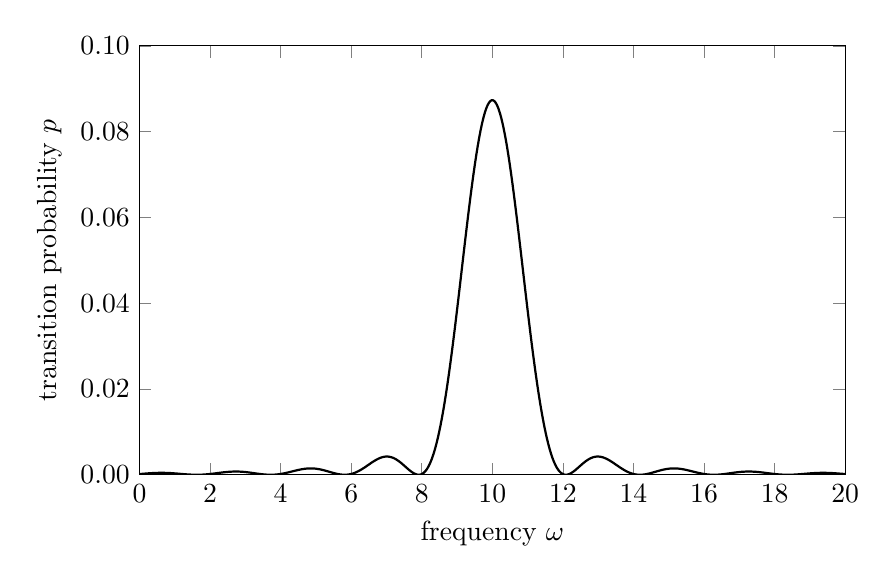
\begin{tikzpicture}
        \begin{axis}[width=300pt, height=200pt, xmin=0.0, xmax=20.0, ymin=0.0, ymax=0.1, xlabel={frequency $\omega$}, ylabel={transition probability $p$}, y tick label style={/pgf/number format/.cd, fixed, fixed zerofill, precision=2, /tikz/.cd }]
        \addplot[color=black, style=thick] coordinates { (0.0, 0.00016789759388031048) (0.03913894324853229, 0.00019273620433729312) (0.07827788649706457, 0.00021808359891844375) (0.11741682974559686, 0.00024361899746823615) (0.15655577299412915, 0.0002690141939291895) (0.19569471624266144, 0.0002939379445829648) (0.23483365949119372, 0.00031806046717407904) (0.273972602739726, 0.00034105799152974847) (0.3131115459882583, 0.0003626173006696379) (0.3522504892367906, 0.00038244020057579366) (0.3913894324853229, 0.0004002478567887186) (0.43052837573385516, 0.000415784936823013) (0.46966731898238745, 0.0004288234990567844) (0.5088062622309197, 0.00043916657123374857) (0.547945205479452, 0.0004466513650048176) (0.5870841487279843, 0.00045115207699565006) (0.6262230919765166, 0.0004525822316755055) (0.6653620352250489, 0.0004508965267682777) (0.7045009784735812, 0.00044609214802615474) (0.7436399217221135, 0.0004382095268083663) (0.7827788649706457, 0.00042733252099196907) (0.821917808219178, 0.00041358800720124746) (0.8610567514677103, 0.00039714488008340306) (0.9001956947162426, 0.0003782124622819231) (0.9393346379647749, 0.0003570383367624975) (0.9784735812133072, 0.0003339056211241765) (1.0176125244618395, 0.00030912971137372517) (1.0567514677103718, 0.00028305453024722935) (1.095890410958904, 0.00025604832242468866) (1.1350293542074363, 0.00022849904579807636) (1.1741682974559686, 0.00020080941422356399) (1.213307240704501, 0.00017339165282140165) (1.2524461839530332, 0.0001466620317972354) (1.2915851272015655, 0.00012103524886920965) (1.3307240704500978, 9.691873362792911e-05) (1.36986301369863, 7.47069494739878e-05) (1.4090019569471623, 5.4775770124065115e-05) (1.4481409001956946, 3.747700801721225e-05) (1.487279843444227, 2.3133171266961446e-05) (1.5264187866927592, 1.2032524083576969e-05) (1.5655577299412915, 4.424522840000794e-06) (1.6046966731898238, 5.156961934505666e-07) (1.643835616438356, 4.6603293515822957e-07) (1.6829745596868884, 4.385935569344972e-06) (1.7221135029354206, 1.233379107846077e-05) (1.761252446183953, 2.431420298658431e-05) (1.8003913894324852, 4.0276920770090706e-05) (1.8395303326810175, 6.011649397850575e-05) (1.8786692759295498, 8.367266922291518e-05) (1.917808219178082, 0.00011073153857700021) (1.9569471624266144, 0.0001410274380367163) (1.9960861056751467, 0.00017424558462438429) (2.035225048923679, 0.00021002543063171407) (2.074363992172211, 0.000247964703506475) (2.1135029354207435, 0.00028762409013296256) (2.152641878669276, 0.0003285325148697043) (2.191780821917808, 0.00037019295181958727) (2.23091976516634, 0.00041208870354359124) (2.2700587084148727, 0.00045369007090995486) (2.309197651663405, 0.0004944613321081581) (2.3483365949119372, 0.0005338679431550117) (2.3874755381604693, 0.0005713838675709731) (2.426614481409002, 0.0006064989393888032) (2.4657534246575343, 0.0006387261613413549) (2.5048923679060664, 0.0006676088390128667) (2.5440313111545985, 0.0006927274519662076) (2.583170254403131, 0.000713706164398095) (2.6223091976516635, 0.0007302188807297922) (2.6614481409001955, 0.0007419947556997281) (2.7005870841487276, 0.0007488230739569232) (2.73972602739726, 0.0007505574208133239) (2.7788649706457926, 0.0007471190736354218) (2.8180039138943247, 0.0007384995522609398) (2.8571428571428568, 0.0007247622767194557) (2.8962818003913893, 0.0007060432913066249) (2.935420743639922, 0.0006825510255866017) (2.974559686888454, 0.0006545650750409991) (3.013698630136986, 0.0006224339966990273) (3.0528375733855184, 0.000586572128017536) (3.091976516634051, 0.0005474554503695243) (3.131115459882583, 0.0005056165315782677) (3.170254403131115, 0.00046163859483140657) (3.2093933463796476, 0.000416148773854325) (3.24853228962818, 0.00036981062624488607) (3.287671232876712, 0.0003233159882061318) (3.326810176125244, 0.00027737626439896515) (3.3659491193737767, 0.00023271325612039934) (3.4050880626223092, 0.00019004963935160868) (3.4442270058708413, 0.00015009921128269268) (3.4833659491193734, 0.00011355702959036019) (3.522504892367906, 8.108957291895331e-05) (3.5616438356164384, 5.332505360946673e-05) (3.6007827788649704, 3.084401466952115e-05) (3.6399217221135025, 1.4170342232819849e-05) (3.679060665362035, 3.7628222938403834e-06) (3.7181996086105675, 7.366317707250772e-09) (3.7573385518590996, 3.2100244337816604e-06) (3.7964774951076317, 1.359089736385619e-05) (3.835616438356164, 3.1279049073210085e-05) (3.8747553816046967, 5.630851144816373e-05) (3.9138943248532287, 8.861546020098975e-05) (3.953033268101761, 0.00012803662780612855) (3.9921722113502933, 0.00017430900472341636) (4.031311154598826, 0.00022707086462481544) (4.070450097847358, 0.00028586413298720733) (4.10958904109589, 0.0003501381014349561) (4.148727984344422, 0.00041925447281437764) (4.187866927592955, 0.0004924937043689937) (4.227005870841487, 0.0005690625987782391) (4.266144814090019, 0.0006481030754458125) (4.305283757338552, 0.0007287020375020136) (4.344422700587084, 0.0008099022337407812) (4.383561643835616, 0.0008907139993670006) (4.422700587084148, 0.0009701277451960638) (4.46183953033268, 0.0010471270520302388) (4.500978473581213, 0.0011207022155268033) (4.540117416829745, 0.0011898640771487996) (4.579256360078277, 0.001253657968911198) (4.61839530332681, 0.0013111775937435836) (4.657534246575342, 0.0013615786595051731) (4.6966731898238745, 0.0014040920831046293) (4.735812133072407, 0.0014380365818664784) (4.774951076320939, 0.0014628304722927254) (4.814090019569472, 0.0014780025017089003) (4.853228962818004, 0.001483201545947117) (4.892367906066536, 0.0014782050161644721) (4.931506849315069, 0.0014629258300543316) (4.970645792563601, 0.001437417816983249) (5.009784735812133, 0.001401879442851954) (5.048923679060665, 0.0013566557585826707) (5.088062622309197, 0.0013022384958988407) (5.12720156555773, 0.0012392642552849172) (5.166340508806262, 0.0011685107534693028) (5.205479452054794, 0.0010908911212181298) (5.244618395303327, 0.0010074462664007267) (5.283757338551859, 0.0009193353419125997) (5.322896281800391, 0.0008278243828318664) (5.362035225048923, 0.000734273201843968) (5.401174168297455, 0.0006401206561969573) (5.440313111545988, 0.0005468684229430319) (5.47945205479452, 0.0004560634416817224) (5.518590998043052, 0.00036927920515128054) (5.557729941291585, 0.00028809609753283175) (5.596868884540117, 0.00021408099796381557) (5.636007827788649, 0.00014876638224783245) (5.6751467710371815, 9.362916886055578e-05) (5.7142857142857135, 5.006956587231622e-05) (5.7534246575342465, 1.939018314998693e-05) (5.7925636007827785, 2.7756790041886288e-06) (5.831702544031311, 1.2732121846447885e-06) (5.870841487279844, 1.577396870124691e-05) (5.909980430528376, 4.699602830055526e-05) (5.949119373776908, 9.546882753270862e-05) (5.98825831702544, 0.0001615194652147821) (6.027397260273972, 0.00024526108178408616) (6.066536203522505, 0.00034658352662701616) (6.105675146771037, 0.00046514650709194845) (6.144814090019569, 0.00060037538971108) (6.183953033268102, 0.0007514597983645276) (6.223091976516634, 0.0009173551259533292) (6.262230919765166, 0.0010967870458707177) (6.301369863013698, 0.0012882590774677253) (6.34050880626223, 0.0014900632261213656) (6.379647749510763, 0.0017002936837761037) (6.418786692759295, 0.001916863540307746) (6.457925636007827, 0.0021375244201350995) (6.49706457925636, 0.0023598889225728724) (6.536203522504892, 0.0025814557088826655) (6.575342465753424, 0.002799637044243473) (6.614481409001956, 0.0030117885693351962) (6.653620352250488, 0.0032152410443092284) (6.692759295499021, 0.00340733377799996) (6.731898238747553, 0.003585449427687292) (6.7710371819960855, 0.0037470498299106837) (6.8101761252446185, 0.0038897125010950427) (6.8493150684931505, 0.004011167428385821) (6.888454011741683, 0.0041093337563815795) (6.927592954990215, 0.004182355964639106) (6.966731898238747, 0.004228639124113285) (7.00587084148728, 0.004246882818244204) (7.045009784735812, 0.00423611331633772) (7.084148727984344, 0.00419571359327734) (7.123287671232877, 0.004125450800482157) (7.162426614481409, 0.004025500808367805) (7.201565557729941, 0.0038964694603053555) (7.240704500978473, 0.0037394102020894397) (7.279843444227005, 0.0035558377790557666) (7.318982387475538, 0.003347737725016555) (7.35812133072407, 0.003117571402851871) (7.397260273972602, 0.0028682763956034752) (7.436399217221135, 0.0026032620889227215) (7.475538160469667, 0.002326400330344657) (7.514677103718199, 0.0020420110976816543) (7.553816046966731, 0.001754843157407113) (7.592954990215263, 0.001470049743760483) (7.632093933463796, 0.001193159339957695) (7.671232876712328, 0.0009300416938261366) (7.71037181996086, 0.0006868692508804608) (7.749510763209393, 0.00047007423778916326) (7.788649706457925, 0.00028630167782451633) (7.8277886497064575, 0.00014235866671995603) (7.86692759295499, 4.5160281868380966e-05) (7.906066536203522, 1.6725394881380236e-06) (7.945205479452055, 1.8852852788662737e-05) (7.984344422700587, 0.00010358847883967936) (8.023483365949119, 0.00026263347237337275) (8.062622309197652, 0.0005025446907519815) (8.101761252446183, 0.0008296174154787813) (8.140900195694716, 0.0012498211716289553) (8.180039138943249, 0.001768736337186823) (8.21917808219178, 0.002391492139309688) (8.258317025440313, 0.003122706633860199) (8.297455968688844, 0.003966429258081142) (8.336594911937377, 0.0049260865340107745) (8.37573385518591, 0.006004431482187404) (8.414872798434441, 0.007203497281473281) (8.454011741682974, 0.008524555681590036) (8.493150684931507, 0.00996808064041825) (8.532289628180038, 0.011533717618544489) (8.571428571428571, 0.013220258919257563) (8.610567514677104, 0.015025625413583191) (8.649706457925635, 0.01694685493742334) (8.688845401174168, 0.01898009759189629) (8.7279843444227, 0.021120618119064048) (8.767123287671232, 0.02336280546392888) (8.806262230919765, 0.025700189570436946) (8.845401174168297, 0.028125465394855356) (8.88454011741683, 0.030630524054882372) (8.92367906066536, 0.03320649096784136) (8.962818003913894, 0.03584377076692754) (9.001956947162427, 0.03853209872133451) (9.041095890410958, 0.04126059832482734) (9.08023483365949, 0.0440178446585342) (9.119373776908024, 0.046791933077998414) (9.158512720156555, 0.04957055272242878) (9.197651663405088, 0.052341064296124805) (9.23679060665362, 0.05509058152873644) (9.275929549902152, 0.05780605568279485) (9.315068493150685, 0.060474362444210776) (9.354207436399216, 0.06308239050454159) (9.393346379647749, 0.06561713112307237) (9.432485322896282, 0.06806576794235827) (9.471624266144813, 0.07041576632303831) (9.510763209393346, 0.07265496146253556) (9.549902152641877, 0.07477164456777219) (9.58904109589041, 0.07675464636422817) (9.628180039138943, 0.07859341724245904) (9.667318982387474, 0.08027810336843913) (9.706457925636007, 0.08179961811557152) (9.74559686888454, 0.08314970821364787) (9.784735812133071, 0.08432101405311249) (9.823874755381604, 0.08530712363128984) (9.863013698630137, 0.08610261968034026) (9.902152641878669, 0.08670311957412184) (9.941291585127201, 0.08710530767232179) (9.980430528375733, 0.08730695982461673) (10.019569471624266, 0.08730695982461671) (10.058708414872799, 0.08710530767232179) (10.09784735812133, 0.08670311957412186) (10.136986301369863, 0.08610261968034026) (10.176125244618394, 0.0853071236312899) (10.215264187866927, 0.08432101405311256) (10.25440313111546, 0.08314970821364787) (10.293542074363991, 0.08179961811557157) (10.332681017612524, 0.08027810336843921) (10.371819960861057, 0.07859341724245904) (10.410958904109588, 0.07675464636422825) (10.450097847358121, 0.07477164456777229) (10.489236790606654, 0.07265496146253556) (10.528375733855185, 0.07041576632303842) (10.567514677103718, 0.06806576794235827) (10.60665362035225, 0.06561713112307246) (10.645792563600782, 0.06308239050454172) (10.684931506849315, 0.060474362444210776) (10.724070450097846, 0.05780605568279499) (10.76320939334638, 0.05509058152873644) (10.80234833659491, 0.05234106429612492) (10.841487279843443, 0.049570552722428905) (10.880626223091976, 0.046791933077998414) (10.919765166340508, 0.04401784465853433) (10.95890410958904, 0.041260598324827466) (10.998043052837573, 0.03853209872133451) (11.037181996086105, 0.03584377076692767) (11.076320939334638, 0.033206490967841486) (11.11545988258317, 0.030630524054882372) (11.154598825831702, 0.028125465394855474) (11.193737769080235, 0.025700189570436946) (11.232876712328766, 0.02336280546392899) (11.272015655577299, 0.02112061811906415) (11.311154598825832, 0.01898009759189629) (11.350293542074363, 0.01694685493742344) (11.389432485322896, 0.015025625413583191) (11.428571428571427, 0.01322025891925764) (11.46771037181996, 0.011533717618544555) (11.506849315068493, 0.00996808064041825) (11.545988258317024, 0.008524555681590098) (11.585127201565557, 0.007203497281473347) (11.62426614481409, 0.006004431482187404) (11.663405088062621, 0.004926086534010819) (11.702544031311154, 0.003966429258081183) (11.741682974559687, 0.003122706633860199) (11.780821917808218, 0.002391492139309719) (11.819960861056751, 0.001768736337186823) (11.859099804305282, 0.0012498211716289768) (11.898238747553815, 0.0008296174154787981) (11.937377690802348, 0.0005025446907519815) (11.97651663405088, 0.00026263347237338186) (12.015655577299412, 0.00010358847883968299) (12.054794520547944, 1.885285278866502e-05) (12.093933463796477, 1.6725394881373711e-06) (12.13307240704501, 4.516028186837936e-05) (12.17221135029354, 0.00014235866671995042) (12.211350293542074, 0.00028630167782451395) (12.250489236790607, 0.00047007423778916326) (12.289628180039138, 0.0006868692508804506) (12.32876712328767, 0.0009300416938261285) (12.367906066536204, 0.001193159339957695) (12.407045009784735, 0.0014700497437604677) (12.446183953033268, 0.001754843157407106) (12.485322896281799, 0.0020420110976816412) (12.524461839530332, 0.002326400330344651) (12.563600782778865, 0.0026032620889227215) (12.602739726027396, 0.0028682763956034635) (12.641878669275929, 0.003117571402851866) (12.68101761252446, 0.00334773772501655) (12.720156555772993, 0.0035558377790557583) (12.759295499021526, 0.003739410202089434) (12.798434442270057, 0.003896469460305348) (12.83757338551859, 0.004025500808367802) (12.876712328767123, 0.004125450800482157) (12.915851272015654, 0.004195713593277337) (12.954990215264187, 0.004236113316337718) (12.99412915851272, 0.004246882818244204) (13.033268101761252, 0.004228639124113288) (13.072407045009784, 0.004182355964639108) (13.111545988258316, 0.004109333756381583) (13.150684931506849, 0.004011167428385824) (13.189823874755382, 0.0038897125010950427) (13.228962818003913, 0.0037470498299106898) (13.268101761252446, 0.0035854494276872967) (13.307240704500977, 0.0034073337779999685) (13.34637964774951, 0.0032152410443092375) (13.385518590998043, 0.0030117885693352014) (13.424657534246574, 0.0027996370442434824) (13.463796477495107, 0.002581455708882669) (13.50293542074364, 0.0023598889225728724) (13.542074363992171, 0.00213752442013511) (13.581213307240704, 0.0019168635403077497) (13.620352250489237, 0.0017002936837761037) (13.659491193737768, 0.0014900632261213773) (13.698630136986301, 0.0012882590774677314) (13.737769080234832, 0.0010967870458707262) (13.776908023483365, 0.000917355125953332) (13.816046966731898, 0.0007514597983645276) (13.85518590998043, 0.0006003753897110864) (13.894324853228962, 0.00046514650709195225) (13.933463796477493, 0.0003465835266270212) (13.972602739726026, 0.00024526108178409033) (14.01174168297456, 0.00016151946521478436) (14.05088062622309, 9.546882753271122e-05) (14.090019569471623, 4.6996028300556447e-05) (14.129158512720156, 1.577396870124691e-05) (14.168297455968688, 1.2732121846451734e-06) (14.20743639921722, 2.775679004188489e-06) (14.246575342465754, 1.939018314998693e-05) (14.285714285714285, 5.006956587231454e-05) (14.324853228962818, 9.362916886055429e-05) (14.363992172211349, 0.00014876638224783166) (14.403131115459882, 0.00021408099796381338) (14.442270058708415, 0.00028809609753283175) (14.481409001956946, 0.0003692792051512753) (14.520547945205479, 0.0004560634416817196) (14.55968688845401, 0.0005468684229430307) (14.598825831702543, 0.0006401206561969546) (14.637964774951076, 0.0007342732018439653) (14.677103718199607, 0.0008278243828318604) (14.71624266144814, 0.0009193353419125967) (14.755381604696673, 0.0010074462664007267) (14.794520547945204, 0.0010908911212181276) (14.833659491193737, 0.0011685107534693002) (14.87279843444227, 0.0012392642552849172) (14.911937377690801, 0.001302238495898838) (14.951076320939334, 0.0013566557585826698) (14.990215264187865, 0.0014018794428519513) (15.029354207436398, 0.0014374178169832494) (15.068493150684931, 0.0014629258300543316) (15.107632093933463, 0.0014782050161644713) (15.146771037181995, 0.0014832015459471171) (15.185909980430527, 0.001478002501708901) (15.22504892367906, 0.0014628304722927267) (15.264187866927593, 0.0014380365818664792) (15.303326810176124, 0.0014040920831046313) (15.342465753424657, 0.0013615786595051742) (15.38160469667319, 0.0013111775937435836) (15.42074363992172, 0.0012536579689112) (15.459882583170254, 0.0011898640771488) (15.499021526418787, 0.0011207022155268033) (15.538160469667318, 0.001047127052030243) (15.57729941291585, 0.000970127745196064) (15.616438356164382, 0.0008907139993670033) (15.655577299412915, 0.0008099022337407838) (15.694716242661448, 0.0007287020375020136) (15.73385518590998, 0.0006481030754458151) (15.772994129158512, 0.0005690625987782392) (15.812133072407043, 0.000492493704368998) (15.851272015655576, 0.00041925447281438176) (15.89041095890411, 0.00035013810143495814) (15.92954990215264, 0.00028586413298720923) (15.968688845401173, 0.0002270708646248171) (16.007827788649706, 0.00017430900472341636) (16.046966731898237, 0.00012803662780612988) (16.08610567514677, 8.861546020099089e-05) (16.125244618395303, 5.630851144816373e-05) (16.164383561643834, 3.1279049073211366e-05) (16.203522504892366, 1.3590897363857037e-05) (16.2426614481409, 3.2100244337816604e-06) (16.28180039138943, 7.366317707250774e-09) (16.320939334637963, 3.762822293840169e-06) (16.360078277886497, 1.4170342232819849e-05) (16.39921722113503, 3.0844014669521164e-05) (16.43835616438356, 5.332505360946519e-05) (16.477495107632095, 8.108957291895331e-05) (16.516634050880626, 0.0001135570295903602) (16.555772994129157, 0.0001500992112826903) (16.594911937377688, 0.00019004963935160616) (16.634050880626223, 0.00023271325612039934) (16.673189823874754, 0.00027737626439896385) (16.712328767123285, 0.0003233159882061289) (16.75146771037182, 0.00036981062624488607) (16.79060665362035, 0.0004161487738543222) (16.829745596868882, 0.0004616385948314024) (16.868884540117417, 0.0005056165315782677) (16.908023483365948, 0.0005474554503695243) (16.94716242661448, 0.0005865721280175336) (16.986301369863014, 0.0006224339966990273) (17.025440313111545, 0.0006545650750409981) (17.064579256360076, 0.0006825510255865999) (17.10371819960861, 0.0007060432913066249) (17.142857142857142, 0.0007247622767194552) (17.181996086105674, 0.0007384995522609388) (17.22113502935421, 0.0007471190736354225) (17.26027397260274, 0.0007505574208133239) (17.29941291585127, 0.0007488230739569234) (17.338551859099802, 0.0007419947556997289) (17.377690802348337, 0.0007302188807297922) (17.416829745596868, 0.000713706164398096) (17.4559686888454, 0.0006927274519662098) (17.495107632093934, 0.0006676088390128667) (17.534246575342465, 0.0006387261613413558) (17.573385518590996, 0.0006064989393888053) (17.61252446183953, 0.0005713838675709731) (17.651663405088062, 0.0005338679431550129) (17.690802348336593, 0.0004944613321081594) (17.729941291585128, 0.00045369007090995486) (17.76908023483366, 0.0004120887035435925) (17.80821917808219, 0.0003701929518195886) (17.84735812133072, 0.00032853251486970674) (17.886497064579256, 0.00028762409013296256) (17.925636007827787, 0.0002479647035064763) (17.96477495107632, 0.00021002543063171632) (18.003913894324853, 0.00017424558462438429) (18.043052837573384, 0.00014102743803671725) (18.082191780821915, 0.0001107315385770011) (18.12133072407045, 8.367266922291518e-05) (18.16046966731898, 6.0116493978506407e-05) (18.199608610567513, 4.027692077009126e-05) (18.238747553816047, 2.431420298658431e-05) (18.27788649706458, 1.233379107846077e-05) (18.31702544031311, 4.385935569345331e-06) (18.356164383561644, 4.6603293515822957e-07) (18.395303326810176, 5.156961934505666e-07) (18.434442270058707, 4.4245228400006205e-06) (18.47358121330724, 1.2032524083576969e-05) (18.512720156555773, 2.3133171266961446e-05) (18.551859099804304, 3.747700801721227e-05) (18.590998043052835, 5.477577012406286e-05) (18.63013698630137, 7.47069494739878e-05) (18.6692759295499, 9.691873362792842e-05) (18.708414872798432, 0.00012103524886920887) (18.747553816046967, 0.0001466620317972354) (18.786692759295498, 0.00017339165282140087) (18.82583170254403, 0.00020080941422356228) (18.864970645792564, 0.00022849904579807636) (18.904109589041095, 0.00025604832242468866) (18.943248532289626, 0.0002830545302472294) (18.98238747553816, 0.00030912971137372517) (19.021526418786692, 0.0003339056211241765) (19.060665362035223, 0.0003570383367624969) (19.099804305283755, 0.00037821246228192195) (19.13894324853229, 0.00039714488008340306) (19.17808219178082, 0.00041358800720124654) (19.21722113502935, 0.0004273325209919684) (19.256360078277886, 0.0004382095268083663) (19.295499021526417, 0.00044609214802615463) (19.33463796477495, 0.00045089652676827733) (19.373776908023483, 0.0004525822316755055) (19.412915851272015, 0.0004511520769956502) (19.452054794520546, 0.000446651365004818) (19.49119373776908, 0.00043916657123374857) (19.53033268101761, 0.0004288234990567844) (19.569471624266143, 0.00041578493682301336) (19.608610567514678, 0.0004002478567887186) (19.64774951076321, 0.00038244020057579366) (19.68688845401174, 0.00036261730066963863) (19.726027397260275, 0.00034105799152974847) (19.765166340508806, 0.00031806046717407904) (19.804305283757337, 0.0002939379445829663) (19.843444227005868, 0.00026901419392919175) (19.882583170254403, 0.00024361899746823615) (19.921722113502934, 0.00021808359891844524) (19.960861056751465, 0.00019273620433729455) (20.0, 0.00016789759388031048) };
        \end{axis}
    \end{tikzpicture} \]
\end{example}

\begin{topic}{lindbladian}{Lindbladian}
    Let a quantum system with Hamiltonian $H$ be given. The \emph{Lindbladian equation} describes the time-evolution of the \tref{mixed-state}{state} $\rho$ of the system as
    \[ \frac{d \rho}{dt} = - \frac{i}{\hbar} [H, \rho] + \sum_{i = 1}^{n} \gamma_i \left( L_i \rho L_i^\dagger - \frac{1}{2} L_i^\dagger L_i \rho - \frac{1}{2} \rho L_i^\dagger L_i \right) \]
    where $L_i$ are the \textit{jump operators} and $\gamma_i \ge 0$ are the \textit{damping rates} describing the dissipative part of the dynamics of the system.
\end{topic}

\begin{topic}{quantum-harmonic-oscillator}{quantum harmonic oscillator}
    The \emph{quantum harmonic oscillator} is the quantum system with Hamiltonian
    \[ H = \tfrac{1}{2} p^2 + \tfrac{1}{2} \omega^2 q^2 \]
    for some $\omega > 0$, where $p$ and $q$ are operators with $[q, p] = i$.

    The operators
    \[ a^\dagger = \sqrt{\frac{\omega}{2}} q - \frac{i}{\sqrt{2 \omega}} p \quad \textup{ and } \quad a = \sqrt{\frac{\omega}{2}} q + \frac{i}{\sqrt{2 \omega}} p \]
    are called the \emph{creation} and \emph{annihilation operators}, respectively, and they satisfy
    \[ \begin{gathered}
        [a, a^\dagger] = 1, \quad H = \tfrac{1}{2} \omega (a a^\dagger + a^\dagger a) = \omega \big( a^\dagger a + \tfrac{1}{2} \big) , \\[5pt]
        [H, a^\dagger] = \omega a^\dagger \quad \textup{ and } \quad [H, a] = - \omega a .
    \end{gathered} \]
    In particular, for any eigenstate $\ket{E}$ of $H$ with energy $E$, that is, $H \ket{E} = E \ket{E}$, it follows that
    \[ H a^\dagger \ket{E} = (E + \omega) a^\dagger \ket{E} \quad \textup{ and } \quad H a \ket{E} = (E - \omega) a \ket{E} . \]
    This yields a ladder of eigenstates of the system with energies
    \[ \ldots, \; E - 2 \omega, \; E - \omega, \; E, \; E + \omega, \; E + 2 \omega, \; \ldots \]
    If the energy is bounded below, there must be a lowest energy state $\ket{0}$ satisfying $a \ket{0} = 0$. From the expression for $H$ in terms of $a^\dagger$ and $a$ follows that
    \[ H \ket{0} = \tfrac{1}{2} \omega \ket{0} \]
    and the states $\ket{n} = (a^\dagger)^n \ket{0}$ (ignoring normalization) satisfy
    \[ H \ket{n} = (n + \tfrac{1}{2}) \omega \ket{n} . \]
\end{topic}

\begin{topic}{von-neumann-entropy}{von Neumann entropy}
    The \emph{von Neumann entropy} of a \tref{mixed-state}{mixed state} $\rho$ of a quantum system is given by
    \[ S = - \tr ( \rho \ln \rho ) = - \sum_i p_i \ln p_i , \]
    where $\rho = \sum_i p_i \ket{\psi_i} \bra{\psi_i}$ for a basis of eigenvectors $\ket{\psi_i}$.
\end{topic}

\begin{topic}{quantum-teleportation}{quantum teleportation}
    \emph{Quantum teleportation} is a process that allows the transfer of quantum information from one location to another using \tref{entangled-state}{entangled} particles and classical communication.
\end{topic}

\begin{example}{quantum-teleportation}
    Suppose Alice wants to send the \tref{COM:qubit}{qubit} state $\alpha \ket{0} + \beta \ket{1}$ to Bob. To do so, Alice shares an \tref{COM:epr-pair}{EPR pair} with Bob (say Alice holds the first qubit and Bob the second). Initially, their joint state is
    \[ (\alpha \ket{0} + \beta \ket{1}) \otimes \frac{1}{\sqrt{2}} (\ket{00} + \ket{11}) \]
    of which Alice holds the first two qubits, and Bob the third. Now, Alice applies a \tref{COM:cnot-gate}{CNOT gate} on her two qubits, after which the joint state is
    \[ \alpha \ket{0} \otimes \frac{1}{\sqrt{2}} (\ket{00} + \ket{11}) + \beta \ket{1} \otimes \frac{1}{\sqrt{2}} (\ket{10} + \ket{01}) . \]
    Next, Alice applies a \tref{COM:hadamard-gate}{Hadamard gate} on her first qubit, after which the joint state is
    \[ \begin{aligned}
        & \tfrac{1}{2} \ket{00} \otimes (\alpha \ket{0} + \beta \ket{1}) \\
        + & \tfrac{1}{2} \ket{01} \otimes (\alpha \ket{1} + \beta \ket{0}) \\
        + & \tfrac{1}{2} \ket{10} \otimes (\alpha \ket{0} - \beta \ket{1}) \\
        + & \tfrac{1}{2} \ket{11} \otimes (\alpha \ket{1} - \beta \ket{0}) .
    \end{aligned} \]
    Alice then measures her two qubits in the standard basis and sends the result to Bob over a classical channel. From these two bits, Bob can infer which gates he must apply to his qubit in order to regain the state $\alpha \ket{0} + \beta \ket{1}$. Specifically, if the second bit is $1$, he applies an \tref{COM:pauli-gates}{$X$-gate}, and if the first bit is $1$, he applies a \tref{COM:pauli-gates}{$Z$-gate}.

    Note that, if the qubit that Alice started with had been entangled,
    \[ \ket{\Psi_0} \otimes \alpha \ket{0} + \ket{\Psi_1} \otimes \beta \ket{1} \]
    then the entanglement will be preserved after `teleportation'. Indeed, in the above derivation one can replace $\alpha$ with $\ket{\Psi_0} \otimes \alpha$ and $\beta$ with $\ket{\Psi_1} \otimes \beta$.
\end{example}

\begin{topic}{adiabatic-theorem}{adiabatic theorem}
    Let $H(t)$ be the time-dependent Hamiltonian of a quantum system. Denote by $\{ \ket{\psi_n(t)} \}$ an orthogonal set of eigenstates of $H(t)$ at any time $t$, with corresponding energies $E_n(t)$. That is, $H(t) \ket{\psi_n(t)} = E_n(t) \ket{\psi_n(t)}$ for all $n$, and $\braket{\psi_m(t)}{\psi_n(t)} = 0$ for all $m \ne n$.

    Write $\psi(t) = \sum_{n} c_n(t) \psi_n(t)$ for the state of the system at any time $t$. The \emph{adiabatic theorem} states that the coefficients $c_n(t)$ can be approximated as
    \[ c_n(t) \approx c_n(0) \exp(i \theta_n(t)) \exp(i \gamma_n(t)) \]
    for $t \ge 0$, where
    \[ \theta_n(t) = - \frac{1}{\hbar} \int_{0}^{t} E_n(s) ds \quad \textup{ and } \quad \gamma_n(t) = i \int_{0}^{t} \braket{\psi_n(s)}{\dot{\psi}_n(s)} ds \]
    are known as the \textit{dynamical phase} and \textit{geometric phase}, respectively.
\end{topic}

\begin{example}{adiabatic-theorem}
    \begin{proof}
        Expanding the time-dependent Schrödinger equation $i \hbar \ket{\dot{\psi}(t)} = H(t) \ket{\psi(t)}$ in terms of the coefficients $c_n(t)$ gives
        \[ i \hbar \left( \dot{c}_n(t) + \sum_{m} c_m(t) \braket{\psi_n(t)}{\dot{\psi}_m(t)} \right) = c_n(t) E_n(t) \]
        for every $n$. On the other hand, the derivative of $H(t) \ket{\psi_m(t)} = E_m(t) \ket{\psi_n(t)}$ with respect to $t$ is
        \[ \dot{H}(t) \ket{\psi_m(t)} + H(t) \ket{\dot{\psi}_m(t)} = \dot{E}_m(t) \ket{\psi_m(t)} + E_m(t) \ket{\dot{\psi}_m(t)} , \]
        whose inner product with $\bra{\psi_n(t)}$ results in
        \[ \braket{\psi_n(t)}{\dot{\psi}_m(t)} = - \frac{\bra{\psi_n(t)} \dot{H}(t) \ket{\psi_m(t)}}{E_n(t) - E_m(t)} \quad \textup{ for all } m \ne n . \]
        Substituting this into the differential equation above gives
        \[ \dot{c}_n(t) + \left( \frac{i}{\hbar} E_n(t) + \braket{\psi_n(t)}{\dot{\psi}_n(t)} \right) c_n(t) = \sum_{m \ne n} \frac{\bra{\psi_n(t)} \dot{H}(t) \ket{\psi_m(t)}}{E_n(t) - E_m(t)} c_m(t) . \]
        Now, if the rate of change $\dot{H}(t)$ is sufficiently small and the energy gaps $|E_n(t) - E_m(t)| > 0$ are sufficiently large, we can neglect the right-hand side of this equation. This is known as the \textit{adiabatic approximation}. Then the equations for the functions $c(t)$ are decoupled and can be solved for to arrive at the statement of the theorem.
    \end{proof}
\end{example}

\begin{example}{adiabatic-theorem}
    Let $H(s)$ be a family of Hamiltonians for $0 \le s \le 1$. Consider a quantum system that evolves under the Hamiltonian $H(t/T)$ from time $t = 0$ to time $t = T$. The time-evolution of this system is then given by the unitary
    \[ \begin{aligned}
        U &= \lim_{N \to \infty} \prod_{k = 0}^{N - 1} \exp \left( - \frac{i}{\hbar} H \left(\tfrac{k \Delta t}{T} \right) \Delta t \right) \quad \textup{ where } \Delta t = T / N \\
        &= \lim_{N \to \infty} \prod_{k = 0}^{N - 1} \exp \left( - \frac{i}{\hbar N} T H \left(\tfrac{k}{N} \right) \right) . 
    \end{aligned} \]
    From this we can see that multiplying the duration $T$ by some factor is equivalent to scaling the Hamiltonian by that same factor. In particular, as $T \to \infty$ the adiabatic approximation becomes valid (as it is equivalent to scaling the energy gaps). 
\end{example}

\begin{topic}{fidelity}{fidelity}
    The \emph{fidelity} between two \tref{density-matrix}{states} $\rho$ and $\sigma$ is
    \[ F(\rho, \sigma) = \left[ \tr \sqrt{\sqrt{\rho} \sigma \sqrt{\rho}} \right]^2 . \]
\end{topic}

\begin{example}{fidelity}
    When $\rho$ and $\sigma$ are \tref{pure-state}{pure states}, that is, $\rho = \ket{\psi} \bra{\psi}$ and $\sigma = \ket{\phi} \bra{\phi}$ for some $\ket{\psi}$ and $\ket{\phi}$, one has $\sqrt{\rho} = \rho$ and $\sqrt{\sigma} = \sigma$, so that the fidelity between $\rho$ and $\sigma$ simplifies to
    \[ F(\rho, \sigma) = \left( \tr \sqrt{\ket{\psi} \braket{\psi}{\phi} \braket{\phi}{\psi} \bra{\psi}} \right)^2 = \left( \sqrt{|\braket{\psi}{\phi}|^2} \tr \sqrt{\ket{\psi} \bra{\psi}} \right)^2 = |\braket{\psi}{\phi}|^2 . \]
\end{example}

\begin{topic}{bell-theorem}{Bell's theorem}
    \emph{Bell's theorem} states that quantum mechanics is incompatible with local realism.
\end{topic}

\begin{example}{bell-theorem}
    Consider the following experiment. Alice and Bob, separated by a great distance, are both given one of two particles that are prepared by Charlie. Upon receiving her particle, Alice will randomly choose whether to measure her particle with measurement $A_1$, yielding outcome $a_1 \pm 1$, or with measurement $A_2$, yielding outcome $a_2 = \pm 1$. Similarly, Bob will randomly choose whether to measure his particle with measurement $B_1$ or $B_2$, yielding outcome $b_1 = \pm 1$ or $b_2 = \pm 2$, respectively.

    Now, consider the expression
    \[ a_1 b_1 + a_1 b_2 + a_2 b_1 - a_2 b_2 . \]
    Under the assumption of local realism, a measurement can only reveal a property that the particle already possessed. In particular, the particles will already have the properties $a_1, a_2, b_1$ and $b_2$ even before measurement. Since for all $a_1, a_2, b_1, b_2 \in \{ \pm 1 \}$ the expression has value $\pm 2$, the expected value of the expression after many repetitions of the experiment should be bounded as follows:
    \[ |\langle A_1 B_1 \rangle + \langle A_1 B_2 \rangle + \langle A_2 B_1 \rangle - \langle A_2 B_2 \rangle| \le 2 \]
    This is known as (an instance of) \textit{Bell's inequality}.

    Finally, let us show that quantum mechanics violates this inequality. Suppose Charlie always prepares a pair of \tref{COM:qubit}{qubits} in the state
    \[ \ket{\Psi^-} = \frac{1}{\sqrt{2}} \left( \ket{0} \otimes \ket{1} - \ket{1} \otimes \ket{0} \right) \]
    of which the first one is sent to Alice, and the second one to Bob, and suppose that Alice's and Bob's measurements are given by
    \[ A_1 = \begin{pmatrix} 1 & 0 \\ 0 & -1 \end{pmatrix}, \quad A_2 = \begin{pmatrix} 0 & 1 \\ 1 & 0 \end{pmatrix}, \quad B_1 = \frac{1}{\sqrt{2}} \begin{pmatrix} -1 & -1 \\ -1 & 1 \end{pmatrix}, \quad B_2 = \frac{1}{\sqrt{2}} \begin{pmatrix} -1 & 1 \\ 1 & 1 \end{pmatrix} . \]
    Then a straight-forward computation shows that
    \[ \bra{\Psi^-} \left( A_1 \otimes B_1  + A_1 \otimes B_2 + A_2 \otimes B_1 - A_2 \otimes B_2 \right) \ket{\Psi^-} = 2 \sqrt{2} \]
    violating Bell's inequality.
\end{example}
